
In this section, we discuss the input/output (I/O) capabilities in Matlab.

\section{Matlab: Input Commands}\label{sec:Matlab_input}

In order to run either script M-files or function M-files, the user needs to provide data, either numerical or text (``strings'').�
The first command we consider is simply called \cour{input}.  \\

\index{Matlab Functions!\cour{input}}
\example{input}{\textbf{Using the \cour{input} command}\\

Here is a simple section of code to collect a person's first name and their age.  \\
\\
\cour{>> FirstName = input({\color{myred} \tq Enter your first name : \tq},{\color{myred} \tq s\tq)}};\\
\cour{>> Age = input({\color{myred}\tq Enter your age : \tq})};\\

Once executed, the user enters values for each, say\\
\\
\cour{Enter your first name : Bob}\\
\cour{Enter your age : 25}
}\\

In this example, the \cour{{\color{myred} \tq s\tq}} in the first \cour{input} indicates that the program expects text input and the second \cour{input} (without the \cour{{\color{myred} \tq s\tq}}) indicates that the program expects numeric input.  When executed, the lines collect input one at a time. Note the text \cour{Waiting for input} on the bottom left of the Matlab window while the user enters the name, \cour{Bob}, and age, \cour{25}. Due to the semicolons, there is no output to the screen, but the values have been stored in the variables \cour{FirstName} and \cour{Age} (see the Workspace window to confirm).

So how do we display this information?  There are several ways to output this information.  Here we consider the two commands \cour{disp} (for ``display'') and \cour{fprintf} (``formated print to file'').  The help files are useful so look them up!\\
�
We can present this information as follows.\\

\index{Matlab Functions!\cour{disp}}
\example{ex_disp}{\textbf{Using the \cour{disp} command}\\

Using the data from the last example:\\
\\
\cour{>> disp({\color{myred} \tq Your first name is \tq})}\\
\cour{>> disp(FirstName)}\\
\cour{>> disp({\color{myred} \tq Your age is \tq})}\\
\cour{>> disp(Age)}\\
\\
which has the output:\\
\\
\cour{Your first name is }\\
\cour{Bob}\\
\cour{Your age is}\\ 
\cour{\ps 25}
}\\

This example is ok, but it would be nicer if the data was in one line.  That's where the command \cour{fprintf} comes in.  Even though it is a formatted print ``to file'' you can have the output sent to the Command Window instead.\\

\index{Matlab Functions!\cour{fprintf}}
\example{ex_fprintf}{\textbf{Using the command \cour{fprintf}}\\


\noindent\cour{>> fprintf({\color{myred} \tq \%s is \%.0f years old.$\backslash$n \tq},FirstName,Age)}\\
\\
produces\\
\\
\cour{Bob is 25 years old.}
}\\

Certainly, there is more involved in the function \cour{fprintf} in order to produce the output we want.  Let's look at the individual pieces of this example.\\
\\
$\bullet$ The \cour{\color{myred}\%} signs are NOT for comments this time (note: they aren't green), they are now used as place holders for the data.\\ 
\\
$\bullet$ The \cour{\color{myred}\%s} indicates that a string is expected as input.\\
\\  
$\bullet$ The \cour{\color{myred}\%.0f} indicates that we expect a numeric input, want zero decimal points and the value should be in Fixed-point format.\\ 
\\
For more information on specific formats and ``conversion characters'' (which is what \cour{\color{myred} f} and \cour{\color{myred} s} are here), look at the \cour{fprintf} command in the help files.  \\
\\
$\bullet$ The {\color{myred} $\backslash$n} is an ``escape character'' that creates a New Line.\\
\\
$\bullet$ The data \cour{FirstName} and \cour{Age} are listed after this, separated by commas.\\
\\
$\bullet$ When the command is run, Matlab places the first data value, \cour{FirstName} (i.e. \cour{Bob}), in the \cour{\color{myred}\%s} position and the second data value, \cour{Age} (i.e. \cour{25}), in the \cour{\color{myred}\%.0f} position.  Got it?\\

Just for completeness, we can also force the \cour{disp} command to act like \cour{fprintf} as follows:\\

\example{ex_dispfprintf}{\textbf{\cour{disp} using concatenated strings}\\
\\
\cour{>> disp([FirstName,{\color{myred} \tq \po is \tq}, num2str(Age),{\color{myred} \tq \po years old.\tq}])}\\
\\
produces\\
\\
\cour{Bob is 25 years old.}
}\\

\index{Matlab Functions!\cour{num2str}}
Basically, we are displaying a string array made up of several strings through concatenation.  We also see the command \cour{num2str} which does exactly what it says, it converts a number into a string.  This is necessary since numeric data and strings don't play well together in Matlab.  In order to create a string array, all of the parts must be strings.  If we tried to run this without the \cour{num2str} command, we would get\\
\\
\cour{>> disp([FirstName,{\color{myred} \tq \po is \tq}, Age,{\color{myred} \tq \po years old.\tq}])}\\
\\
with output\\
\\
\cour{Bob is $\square$ years old.}\\
\\
where the square indicates that the ASCII code for the value 25 is unprintable (look it up or don't worry about it - just remember the \cour{num2str}).\\

Let's look at how to read and write larger data files next.\\

\example{ex_steeldata}{\po\\

Create the following table of years and monthly world steel production (in thousand metric tons) in an Excel file and save the file as WorldSteelProduction.xls (or .xlsx).  Make sure to save this file in the directory listed at the top of the Matlab window, the Currect Directory.

\begin{center}
\begin{tabular}{|c|c|c|c|c|c|}
\hline
{\bf 2005}&	{\bf 2006}	&{\bf 2007}&	{\bf 2008}&	{\bf 2009}&	{\bf 2010}\\ \hline
91377&	95037&	107789&	112870&	86476&	113375\\ \hline
84980&	91183&	101465&	107465&	86610&	107119\\ \hline
93198&	102183&	112988&	119934&	92144&	122196\\ \hline
93381&	101604&	110241&	117023&	89644&	120497\\ \hline
95290&	105501&	112933&	121062&	96177&	124567\\ \hline
92095&	104636&	112159&	118851&	100661&	118346\\ \hline
90205&	104350&	110377&	116770&	104701&	114365\\ \hline
91536&	102630&	109024&	112726&	108351&	113141\\ \hline
93144&	103676&	111956&	107723&	110773&	112340\\ \hline
98534&	106913&	114703&	99202&	114765&	117377\\ \hline
94340&	104817&	109936&	86513&	108596&	114637\\ \hline
95368&	105306&	111506&	81704&	107792&	116157\\
\hline
\end{tabular}
\end{center}

\drawexampleline%{ex_steeldataline}

\index{Matlab Functions!\cour{xlsread}}
\index{Matlab Functions!\cour{ginput}}
\index{Matlab Functions!\cour{legend}}
We will now read in this data using \cour{xlsread}, plot it, and access data from it using the mouse and the graphical input command \cour{ginput} (``gee-input'').\\
\\ \cour{>> Steel = xlsread({\color{myred} \tq WorldSteelProduction.xls\tq});}\\

Next, we plot the data \\
\\
\cour {>> plot(1:12,Steel(2:end,:))}\\
\cour {>> legend({\color{myred} \tq2005\tq,\tq2006\tq,\tq2007\tq,\tq2008\tq,\tq2009\tq,\tq2010\tq, ...}} \\
\indent \cour {{\color{myred} \tq Location\tq,\tq best\tq})}\\
\\

The initial problem is to find the first time in 2009 that steel production is at 100,000 thousand metric tons.  We use the \cour{ginput} command for the user to collect this data.  \\
\\
\cour {>> disp({\color{myred} \tq Select the 2009 time when production is 100,000.\tq});}\\
\cour {>> [t,l] = ginput(1) \color{mygreen} \% mouse click}\\

If the user hovers the cursor over the resulting plot, we see cross-hairs appear:\\

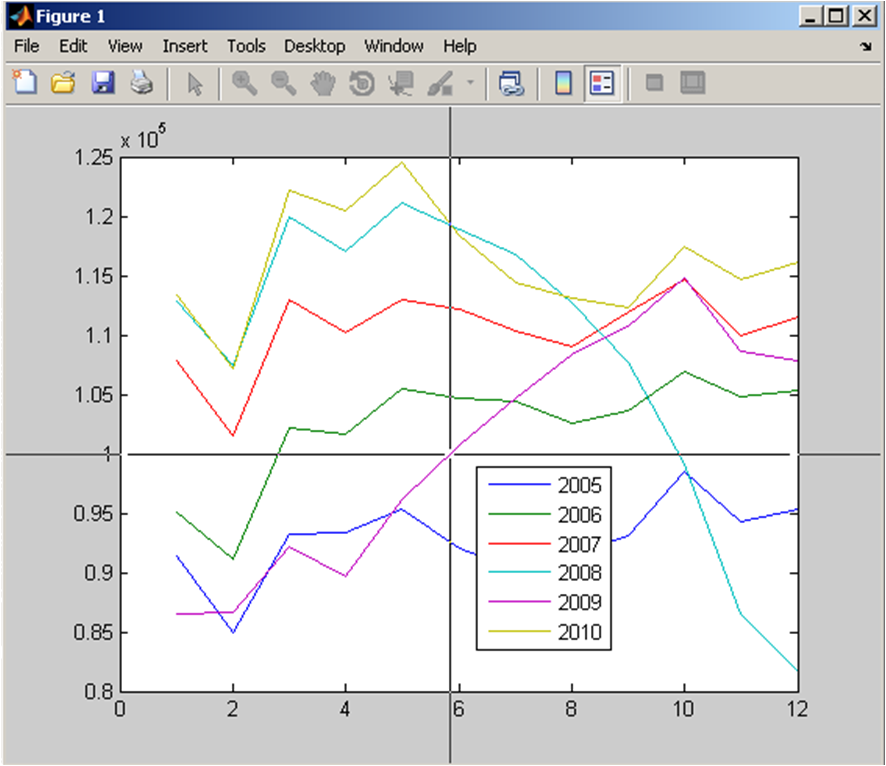
\includegraphics[scale=.7]{figures/matlab_ginput2.png}



A left-click creates the output to appear in the Command Window:\\
\\
\cour{t =}\\
\cour{\ps 5.8756}\\
\cour{l =}\\
\cour{\ps 9.9934e+004}\\

Note that the level is listed in engineering format.  If we want to finish this example with a formatted output, we could use the following:\\
\\
\cour{>> fprintf({\color{myred} \tq Level \%6.1f occurs \%3.1f months into 2009.$\backslash$n\tq},l,t)}\\
\\
\cour{Level 99934.2 occurs 5.9 months into 2009.}\\
\\
which is in mid-June 2009.  Note that the accuracy of the level and time are dependent on the user's mouse click so the output may not look exactly the same.\\
(Data from \cour{http://www.worldsteel.org/})
}\\

\keyidea{idea:matrixfprintf}{\textbf{\cour{fprintf} with matrices}\\
If there are not enough place holders, \cour{fprintf} will cycle through the values in the given data matrix, USING COLUMN PRECEDENCE, until all of the values are exhausted.}


\example{ex_fprintfmatrix}{\po\\

Here we use \cour{fprintf} and Key Idea \ref{idea:matrixfprintf} to display a matrix of values. Find the sine, cosine and tangent of
theta from 0 to $2\pi$ by steps of $\pi/10$.\\
\\
\cour{>> theta=[0:pi/10:2*pi];}\\
\cour{>> values=[theta;sin(theta);cos(theta);tan(theta)];}\\
\\
To display these, we can use a simple \cour{fprintf}. \\
\\
\cour{>> disp({\color{myred} \tq Theta   Sine   Cosine   Tangent \tq});}\\
\cour{>> fprintf(\color{myred} \tq \%5.2f \%6.2f \%7.2f \%9.2f$\backslash$ n \tq,values)}\\
\\
gives output:\\
\\
\cour{Theta  \po \po Sine  \po \po Cosine \po \po  Tangent}\\
 \cour{\po 0.00   \po\po0.00   \po\po 1.00     \phantom{00000} 0.00 }\\
 \cour{\po0.31   \po\po0.31    \po\po0.95      \phantom{000000}0.32 }\\
 \cour{\po0.63   \po\po0.59    \po\po0.81      \phantom{000000}0.73 }\\
 \cour{\po0.94   \po\po0.81    \po\po0.59      \phantom{000000}1.38 }\\
 \cour{\po1.26   \po\po0.95    \po\po0.31      \phantom{000000}3.08 }\\
 \cour{\po1.57   \po\po1.00    \po\po0.00 16331239353195370.00 }\\
 \cour{\po1.88   \po\po0.95   \po-0.31     \phantom{00000}-3.08 }\\
 \cour{\po2.20   \po\po0.81   \po-0.59     \phantom{00000}-1.38 }\\
 \cour{\po2.51   \po\po0.59   \po-0.81     \phantom{00000}-0.73 }\\
 \cour{\po2.83   \po\po0.31   \po-0.95     \phantom{00000}-0.32 }\\
 \cour{\po3.14   \po\po0.00   \po-1.00     \phantom{00000}-0.00 }\\
 \cour{\po3.46  \po-0.31   \po-0.95      \phantom{000000}0.32 }\\
 \cour{\po3.77  \po-0.59   \po-0.81      \phantom{000000}0.73 }\\
 \cour{\po4.08  \po-0.81   \po-0.59      \phantom{000000}1.38 }\\
 \cour{\po4.40  \po-0.95   \po-0.31      \phantom{000000}3.08 }\\
 \cour{\po4.71  \po-1.00   \po-0.00 5443746451065123.00 }\\
 \cour{\po5.03  \po-0.95    \po\po0.31     \phantom{00000}-3.08 }\\
 \cour{\po5.34  \po-0.81    \po\po0.59     \phantom{00000}-1.38 }\\
 \cour{\po5.65  \po-0.59    \po\po0.81     \phantom{00000}-0.73 }\\
 \cour{\po5.97  \po-0.31    \po\po0.95     \phantom{00000}-0.32 }\\
 \cour{\po6.28  \po-0.00    \po\po1.00     \phantom{00000}-0.00 }
}\\

In this example, the reason for the large values in the last column are because the tangent function tends to infinity as the angle tends to $\pi/2$ (and 1.5708 is close to $\pi/2$).  Actually, the value $\tan(\pi/2)$ returns \cour{1.6331e+016}.  Why isn't ``infinity'' the returned value?  Well, it has to do with how values are stored in Matlab (using double-precision).  The value \cour{1.6331e+016} is actually the reciprocal of the value \cour{eps = 10$\wedge$(-52)}.  If you want to know more, head to the help files (or Google, of course).\\


\newpage
\printexercises{exercises/06_exercises}

%\\
%\vspace{1in}
%EXERCISES:\\
%1)For this problem, you will modify your projectile motion function, $<$vmiid$>$ProjMotion, from the last homework.  Now, as part of your function, plot the height from 0 to 30 seconds, use \cour{ginput} to get maximum height and use \cour{fprintf} to display a sentence describing the maximum height and corresponding time.
%\vspace{1in}
%2) For this problem, modify your conversion function from the previous homework and include \cour{fprintf} in order to create a nice-looking table showing conversions between \cour{Dollar, Euro, Yen, and British Pounds}.  
%Include a header for each column and use 0 to 100 dollars in increments of 5.



%\definition{def:lineintegral}{\textbf{TITLE}}
%
%\keyidea{idea:lineintprops}{\textbf{TITLE}}
%
%\printexercises{exercises/mathcad_introduction_exercises}
